\chapter{Modelagem computacional}

Neste capítulo serão apresentados os aspectos para o desenvolvimento da ferramenta, como os pré-requisitos, escolhas das ferramentas, decisões de modelagem, e as práticas adotadas no processo.

%%%%%%%%%%%%%%%%%%%%%%%%%%%%%%%%%%%%%%%%%%%%%%%%%%%%%%%%%%%%%%%%%%%%%%%%%%%%%%%%
% \section{Requisitos da ferramenta}
O levantamento dos requisitos de um sistema é o elemento que fornece elementos que dever nortear uma série de decisões a serem tomadas no seu desenvolvimento.
A ferramenta a ser implementada se propõe:
\begin{itemize}
    \item A partir de um arquivo de entrada com informações do modelo, criar arquivos de entrada para o Abaqus (\texttt{.inp}) que simulem todo o processo de simulação do comportamento do duto apresentado (\autoref{chap:assentamento}).
    \item Processar os arquivos de saída do Abaqus (\texttt{.odb}) extraindo os informações relevantes como a configuração deformada, modos de vibração, etc., gerando arquivos em outros formatos de fácil leitura para pós-processamento, tanto por esta ferramenta, quando por outro \textit{softwares}.
    \item Pós-processar as as informações gerando gráficos e relatórios relevantes para as tomadas de decisão do usuário quanto ao projeto.
\end{itemize}

% \section{Boas práticas para computação científica}

Embora o uso e desenvolvimento de softwares de cunho científico seja uma atividade extremamente importante para pesquisadores, nem sempre são observadas boas práticas são observadas no seu desenvolvimento~\cite{Hannay2009}.
\citeonline{Wilson2014} apresenta um conjunto de boas práticas a serem adotadas no desenvolvimento desse tipo de. A seguir é apresentado o resumo do autor sobre essas práticas:

\vspace{0.5cm}
\begin{tcolorbox}[breakable, enhanced]

\textbf{Boas práticas para computação científica}

\begin{enumerate}
\item \textbf{Escreva programas para pessoas, não para computadores.}
    \begin{enumerate}
        \item Um programa não deve exigir que seus leitores mantenham mais de um punhado de fatos na memória de uma só vez.
        \item Torne os nomes consistentes, distintos e significativos.
        \item Tornar consistente o estilo e a formatação do código.
    \end{enumerate}

\item \textbf{Deixe o computador fazer o trabalho.}
    \begin{enumerate}
        \item Faça o computador repetir tarefas.
        \item Salve comandos recentes em um arquivo para reutilização.
        \item Use uma ferramenta de construção para automatizar fluxos de trabalho.
    \end{enumerate}

\item \textbf{Faça alterações incrementais.}
    \begin{enumerate}
        \item Trabalhe em pequenos passos com feedback frequente e correção de rumo.
        \item Use um sistema de controle de versão.
        \item Coloque tudo o que foi criado manualmente no controle de versão.
    \end{enumerate}

\item \textbf{Não se repita (ou repita outros).}
    \begin{enumerate}
        \item Todos os dados devem ter uma única representação oficial no sistema.
        \item Modularize o código em vez de copiar e colar.
        \item Reutilize o código em vez de reescrevê-lo.
    \end{enumerate}

\item \textbf{Planeje erros.}
    \begin{enumerate}
        \item Adicione asserções aos programas para verificar seu funcionamento.
        \item Use uma biblioteca de testes unitários pronta para uso.
        \item Transforme erros em casos de teste.
        \item Use um depurador simbólico.
    \end{enumerate}

\item \textbf{Otimize o software somente depois que ele funcionar corretamente.}
    \begin{enumerate}
        \item Use um \textit{profiler} para identificar gargalos.
        \item Escreva o código na linguagem de nível mais alto possível.
    \end{enumerate}

\item \textbf{Documente design e finalidade, não a mecânica.}
    \begin{enumerate}
        \item Documente interfaces e razões, não implementações.
        \item Refatore o código, em vez de explicar como ele funciona.
        \item Incorpore a documentação do software no próprio software.
    \end{enumerate}

\item \textbf{Colabore.}
    \begin{enumerate}
        \item Use revisões de código de pré-\textit{merge}.
        \item Use a programação em pares ao interar alguém novo e ao lidar com problemas particularmente difíceis.
        \item Use uma ferramenta de acompanhamento de problemas.
    \end{enumerate}
\end{enumerate}
\end{tcolorbox}

Em observância à estas práticas, algumas decisões foram tomadas quanto ao desenvolvimento da ferramenta, e serão apresentadas a seguir.


% \subsection{}

\begin{itemize}

\item Paradigma de programação

O uso de Programação Orientada a Objeto promove um alto índice de reaproveitamento de código, que vai da direção do item 4 apresentado.

\item Linguagem de programação

A linguagem adotada será Python\footnote{https://www.python.org}. \citeonline{Rao2018} apresenta algumas das principais vantagens que destaca a linguagem para este tipo de aplicação:

\begin{itemize}
    \item Disponibilidade de bibliotecas para aplicações cientificas contemplando manipulação de matrizes (Numpy), funções matemáticas (SciPy), manipulação de dados em forma tabular (Pandas), criação de gráficos interativos (Matplotlib e Bokeh);
    
    \begin{figure}[!ht]
        \centering
        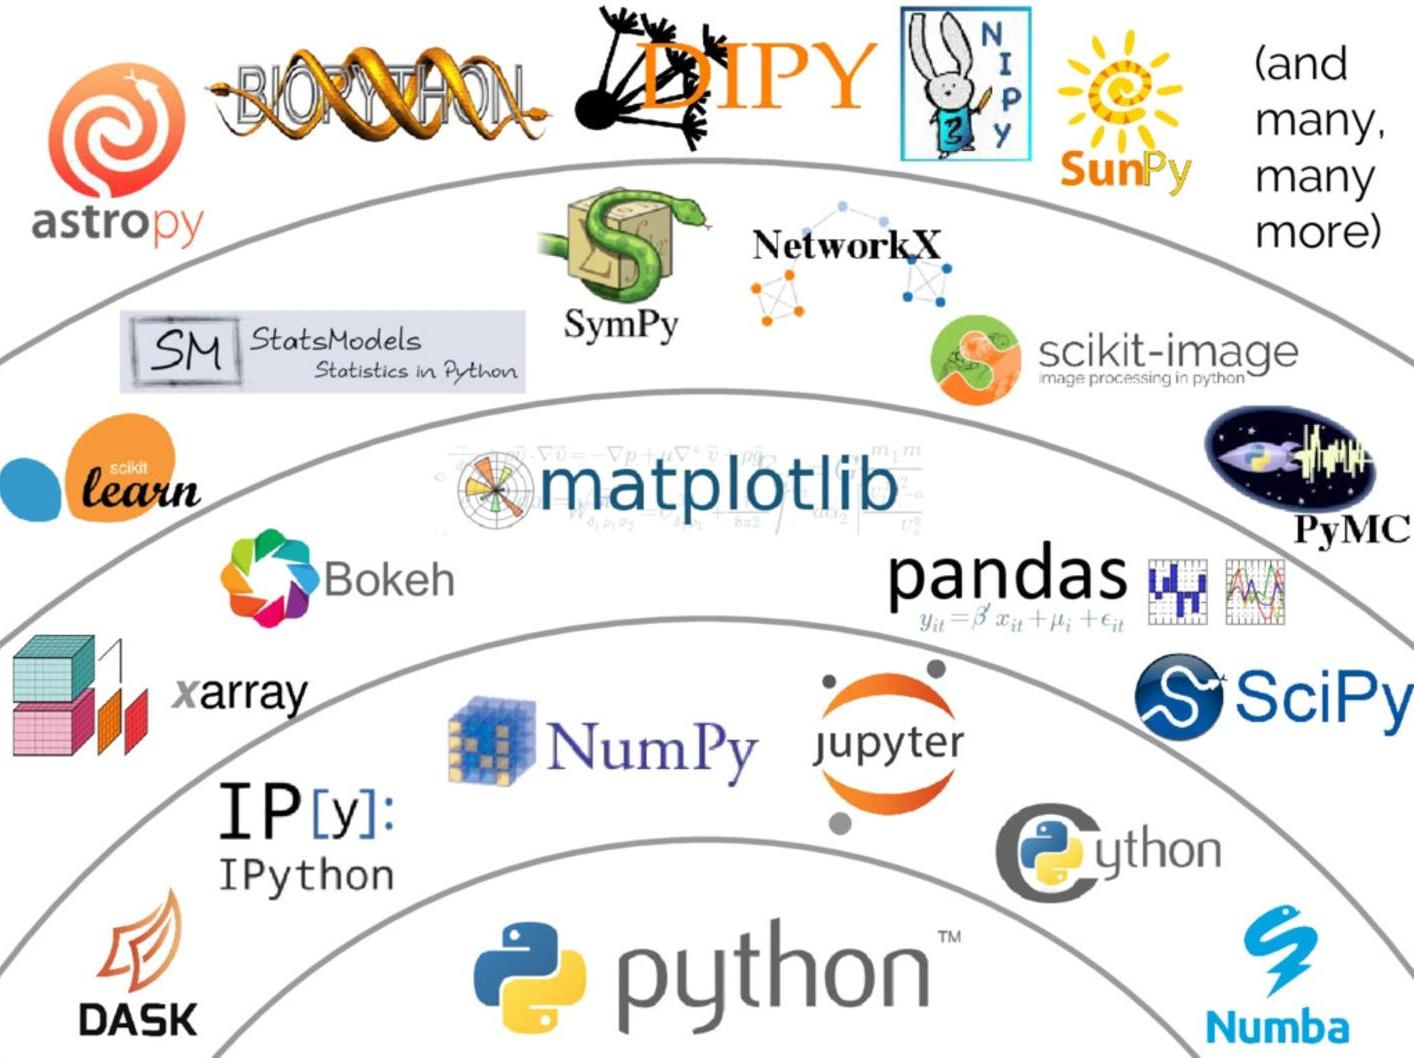
\includegraphics[width=0.6\textwidth]{imagens/python_ecosystem}
        \caption[Amostra das principais bibliotecas científicas em Python]{Amostra das principais bibliotecas científicas em Python.}\label{fig:python_ecosystem}
    \end{figure}

    \item 
\end{itemize}
\end{itemize}
